%%%%%%%%%%%%%%%%%%%%%%%%%%%%%%%%%%%%%%%%%
% a0poster Portrait Poster
% LaTeX Template
% Version 1.0 (22/06/13)
%
% The a0poster class was created by:
% Gerlinde Kettl and Matthias Weiser (tex@kettl.de)
% 
% This template has been downloaded from:
% http://www.LaTeXTemplates.com
%
% License:
% CC BY-NC-SA 3.0 (http://creativecommons.org/licenses/by-nc-sa/3.0/)
%
%%%%%%%%%%%%%%%%%%%%%%%%%%%%%%%%%%%%%%%%%

%----------------------------------------------------------------------------------------
%	PACKAGES AND OTHER DOCUMENT CONFIGURATIONS
%----------------------------------------------------------------------------------------

\documentclass[a0,portrait]{a0poster}

\usepackage{multicol} % This is so we can have multiple columns of text side-by-side
\columnsep=100pt % This is the amount of white space between the columns in the poster
\columnseprule=3pt % This is the thickness of the black line between the columns in the poster

\usepackage[svgnames]{xcolor} % Specify colors by their 'svgnames', for a full list of all colors available see here: http://www.latextemplates.com/svgnames-colors

\usepackage{times} % Use the times font
%\usepackage{palatino} % Uncomment to use the Palatino font

\usepackage{graphicx} % Required for including images
\graphicspath{{../tex/imgs/}} % Location of the graphics files
\usepackage{booktabs} % Top and bottom rules for table
\usepackage[font=small,labelfont=bf]{caption} % Required for specifying captions to tables and figures
\usepackage{amsfonts, amsmath, amsthm, amssymb} % For math fonts, symbols and environments
\usepackage{wrapfig} % Allows wrapping text around tables and figures

% To use subfigure
\usepackage{caption}
\usepackage{subcaption}


\newcommand{\brasaoufes}{
  
\includegraphics[width=4cm]{../../brasao-ufes}
}

\begin{document}

%----------------------------------------------------------------------------------------
%	POSTER HEADER 
%----------------------------------------------------------------------------------------

% The header is divided into two boxes:
% The first is 75% wide and houses the title, subtitle, names, university/organization and contact information
% The second is 25% wide and houses a logo for your university/organization or a photo of you
% The widths of these boxes can be easily edited to accommodate your content as you see fit

\begin{minipage}[c]{0.70\linewidth}
\veryHuge \color{NavyBlue} \textbf{A shuffled complex evolution algorithm for
the multidimensional knapsack problem} \color{Black} % Title
\end{minipage}
\begin{minipage}[c]{0.30\linewidth}
  %\hspace{0.25\linewidth}
  \hfill
  
\includegraphics[scale=2.5]{ciarp-logo}
\end{minipage}\\[1cm]

\begin{minipage}[c]{0.10\linewidth}
  \vspace{-15mm}
  
\includegraphics[scale=1.5]{../../brasao-ufes}
\end{minipage}
\begin{minipage}[c]{0.80\linewidth}
  \huge \textbf{Marcos Baroni \& Fl\'avio Varej\~ao}\\[0.5cm] % Author(s)
  \huge Universidade Federal do Espírito Santo - Departamento de Inform\'atica\\[0.4cm] % University/organization
  \Large \texttt{marcos.baroni@aluno.ufes.br}\\
\end{minipage}

%\vspace{1cm} % A bit of extra whitespace between the header and poster content

%----------------------------------------------------------------------------------------

\begin{multicols}{2} % This is how many columns your poster will be broken into, a portrait poster is generally split into 2 columns

%----------------------------------------------------------------------------------------
%	ABSTRACT
%----------------------------------------------------------------------------------------

\color{Navy} % Navy color for the abstract

\begin{abstract}

This work addresses the application of
a population based evolutionary algorithm
called shuffled complex evolution (SCE) in the multidimensional knapsack
problem.
The SCE regards a natural evolution happening simultaneously in independent communities.
The performance of the SCE algorithm is verified through computational experiments
using well-known problems from literature and randomly generated problem as well.
The SCE proved to be very effective in finding good solutions demanding a
very small amount of processing time. \\
{ \bf Multidimensional knapsack problem, Meta-heuristics, Artificial Intelligence}

\end{abstract}

%----------------------------------------------------------------------------------------
%	INTRODUCTION
%----------------------------------------------------------------------------------------

\color{SaddleBrown} % SaddleBrown color for the introduction

\section*{Introduction}

Aliquam non lacus dolor, \textit{a aliquam quam} \cite{Smith:2012qr}. Cum sociis natoque penatibus et magnis dis parturient montes, nascetur ridiculus mus. Nulla in nibh mauris. Donec vel ligula nisi, a lacinia arcu. Sed mi dui, malesuada vel consectetur et, egestas porta nisi. Sed eleifend pharetra dolor, et dapibus est vulputate eu. \textbf{Integer faucibus elementum felis vitae fringilla.} In hac habitasse platea dictumst. Duis tristique rutrum nisl, nec vulputate elit porta ut. Donec sodales sollicitudin turpis sed convallis. Etiam mauris ligula, blandit adipiscing condimentum eu, dapibus pellentesque risus.

\textit{Aliquam auctor}, metus id ultrices porta, risus enim cursus sapien, quis iaculis sapien tortor sed odio. Mauris ante orci, euismod vitae tincidunt eu, porta ut neque. Aenean sapien est, viverra vel lacinia nec, venenatis eu nulla. Maecenas ut nunc nibh, et tempus libero. Aenean vitae risus ante. Pellentesque condimentum dui. Etiam sagittis purus non tellus tempor volutpat. Donec et dui non massa tristique adipiscing.

%----------------------------------------------------------------------------------------
%	OBJECTIVES
%----------------------------------------------------------------------------------------

\color{DarkSlateGray} % DarkSlateGray color for the rest of the content

\section*{Main Objectives}

\begin{enumerate}
\item Lorem ipsum dolor sit amet, consectetur.
\item Nullam at mi nisl. Vestibulum est purus, ultricies cursus volutpat sit amet, vestibulum eu.
\item Praesent tortor libero, vulputate quis elementum a, iaculis.
\item Phasellus a quam mauris, non varius mauris. Fusce tristique, enim tempor varius porta, elit purus commodo velit, pretium mattis ligula nisl nec ante.
\item Ut adipiscing accumsan sapien, sit amet pretium.
\item Estibulum est purus, ultricies cursus volutpat
\item Nullam at mi nisl. Vestibulum est purus, ultricies cursus volutpat sit amet, vestibulum eu.
\item Praesent tortor libero, vulputate quis elementum a, iaculis.
\end{enumerate}

\begin{figure}
  \begin{subfigure}[t]{0.48\textwidth}
    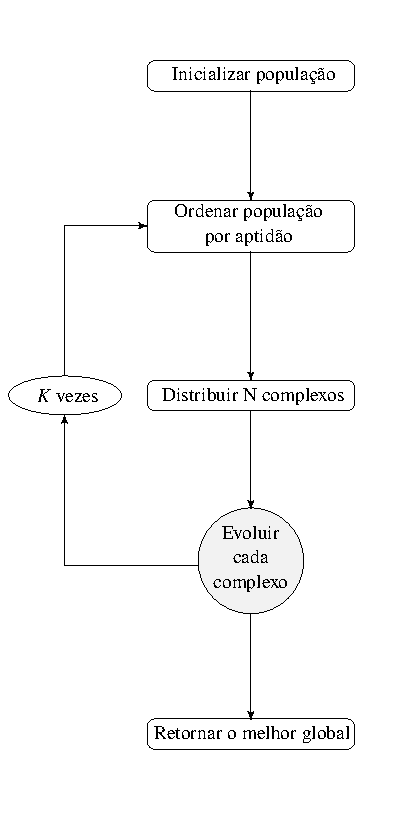
\includegraphics[scale=1.5]{flow1}
  \end{subfigure}
  \begin{subfigure}[t]{0.48\textwidth}
    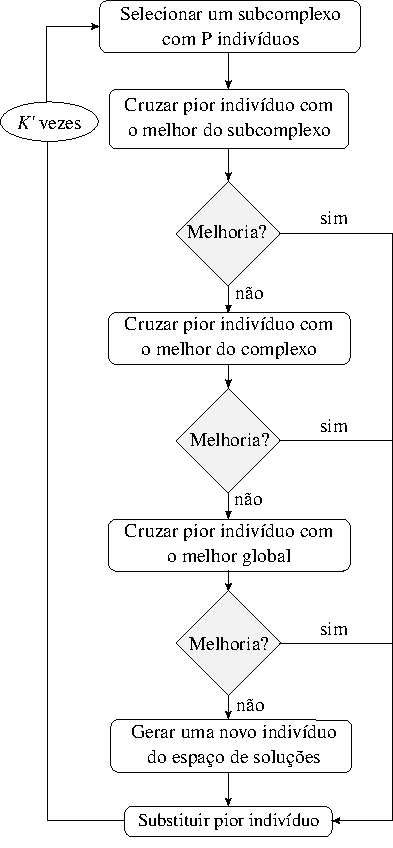
\includegraphics[scale=1.5]{flow2}
  \end{subfigure}
\end{figure}

\begin{center}
\begin{minipage}{0.3\linewidth}
    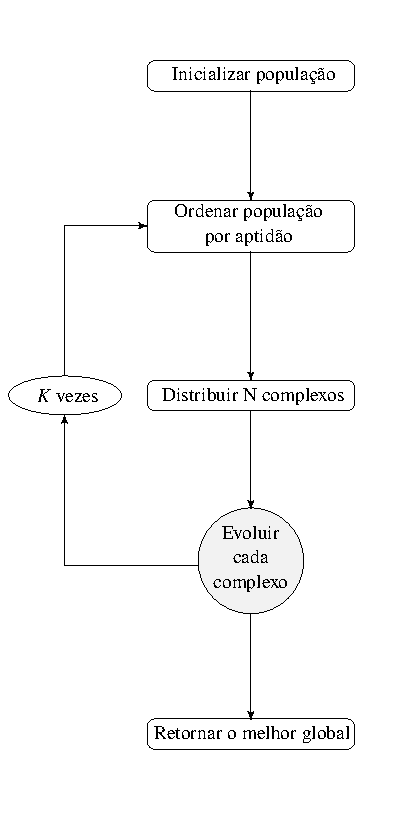
\includegraphics[scale=1.5]{flow1}
\end{minipage}
\begin{minipage}{0.3\linewidth}
    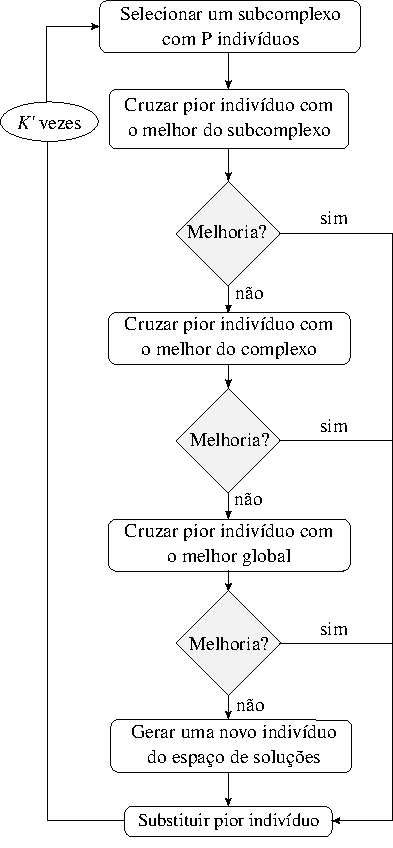
\includegraphics[scale=1.5]{flow2}
\end{minipage}
\end{center}

\color{SaddleBrown} % SaddleBrown color for the conclusions to make them stand out

\section*{Conclusions}

\begin{itemize}
\item Pellentesque eget orci eros. Fusce ultricies, tellus et pellentesque fringilla, ante massa luctus libero, quis tristique purus urna nec nibh. Phasellus fermentum rutrum elementum. Nam quis justo lectus.
\item Vestibulum sem ante, hendrerit a gravida ac, blandit quis magna.
\item Donec sem metus, facilisis at condimentum eget, vehicula ut massa. Morbi consequat, diam sed convallis tincidunt, arcu nunc.
\item Nunc at convallis urna. isus ante. Pellentesque condimentum dui. Etiam sagittis purus non tellus tempor volutpat. Donec et dui non massa tristique adipiscing.
\end{itemize}

\color{DarkSlateGray} % Set the color back to DarkSlateGray for the rest of the content

%----------------------------------------------------------------------------------------
%	FORTHCOMING RESEARCH
%----------------------------------------------------------------------------------------

\section*{Forthcoming Research}

\nocite{*} % Print all references regardless of whether they were cited in the poster or not
\bibliographystyle{plain} % Plain referencing style
\bibliography{sample} % Use the example bibliography file sample.bib


\section*{Acknowledgements}

\end{multicols}

\end{document}
